\documentclass[withoutpreface,bwprint]{cumcmthesis} %去掉封面与编号页
\title{实验报告-实验二}
\author{18340206张德龙 \\
	zhangdlong3@mail2.sysu.edu.cn
}
\date{\today}
\usepackage[cache=false]{minted}
\usepackage{diagbox}
%\usepackage{fancyhdr}
%\pagestyle{empty} 
{\renewcommand\fcolorbox[4][]{\textcolor{cyan}{\strut#4}} %屏蔽汇编语言mint的错误
\graphicspath{{figure/}}

\let\algorithm\relax  
\let\endalgorithm\relax 
\usepackage[linesnumbered,ruled,lined]{algorithm2e}
\usepackage{algpseudocode}  
\renewcommand{\algorithmicrequire}{\textbf{Input:}}   
\renewcommand{\algorithmicensure}{\textbf{Output:}}   
\SetKwFor{For}{for}{do}{endfor}
\newcommand{\ret}{\textbf{return}}   

\makeatletter
\newenvironment{breakablealgorithm}
{% \begin{breakablealgorithm}
	\begin{center}
		\refstepcounter{algorithm}% New algorithm
		\hrule height.8pt depth0pt \kern2pt% \@fs@pre for \@fs@ruled
		\renewcommand{\caption}[2][\relax]{% Make a new \caption
			{\raggedright\textbf{\ALG@name~\thealgorithm} ##2\par}%
			\ifx\relax##1\relax % #1 is \relax
			\addcontentsline{loa}{algorithm}{\protect\numberline{\thealgorithm}##2}%
			\else % #1 is not \relax
			\addcontentsline{loa}{algorithm}{\protect\numberline{\thealgorithm}##1}%
			\fi
			\kern2pt\hrule\kern2pt
		}
	}{% \end{breakablealgorithm}
		\kern2pt\hrule\relax% \@fs@post for \@fs@ruled
	\end{center}
}
\makeatother

\newcounter{Emp}[subsubsection]	% 设置计数器
\newcommand{\kuohao}{\addtocounter{Emp}{1} \noindent (\theEmp)}

\usepackage{amssymb}% http://ctan.org/pkg/amssymb
\usepackage{pifont}% http://ctan.org/pkg/pifont
\newcommand{\cmark}{\ding{51}}%
\newcommand{\xmark}{\ding{55}}%

\usepackage{threeparttable}

\begin{document}
\maketitle
\begin{abstract}
 
 在本次实验中,我们小组完成了三层BP网络的错误反传算法,实现了百分之70以上的准确率。同时,我们就优化器、批量归一化、丢弃法等BP神经网络常见优化方法进行了探究。%hc
 \keywords{BP神经网络 \quad 卷积神经网络 \quad 批量归一化 \quad 丢弃法}
\end{abstract}

\section{导言}

构造一个三层的BP神经网络和一个卷积神经网络,完成手写0-9数字的识别:
\begin{enumerate}
\item 设计网络的结构,比如层数,每层的神经元数,单个神经元的输入输出函数;
\item 根据数字识别的任务,设计网络的输入和输出;
\item 实现BP网络错误反传算法,完成神经网络的训练测试,最终识别率达到70\%以上;
\item 数字识别训练集可以自己手工制作,也可以网上下载,要求具有可视化图形界面,能够输入输出。
\item 进一步的,用卷积神经网络实现以上任务,对比深度学习与浅层模型。
\end{enumerate}


\section{实验过程-BP神经网络}
本次BP神经网络的实现借鉴了斯坦福大学CS231n课程作业的代码框架,核心代码都是由我们小组进行实现。
\subsection{前向传播与反向传播}
\subsubsection{前向传播}
仿射变换的前向传播如下,输入为大小$(N, d_1, \cdots, d_k)$的向量,其中$N$为批量大小;仿射变换的矩阵大小为$(D, M)$,其中$D = \prod_{i=1}^{k} d_i$;偏置的矩阵大小为$(M,)$;通过numpy库的reshape接口,经过简单的仿射变换即可将多维输入线性映射到$(N, M)$的大小。利用cache来存储用于后向传播的缓存。
\begin{lstlisting}[language=python]
	def affine_forward(x, w, b):
	    newx = np.reshape(x, (x.shape[0], -1))
	    out = np.dot(newx, w) + b
	    cache = (x, w, b)
	    return out, cache
\end{lstlisting}
对于Relu函数的前向传播同理:
\begin{lstlisting}[language=python]
	def relu_forward(x):
	    out = np.maximum(x, 0)
	    cache = x
	    return out, cache
\end{lstlisting}


\subsubsection{后向传播}
根据链式法则分别计算对于x、w、b的偏导返回即可:
\begin{lstlisting}[language=python]
	def affine_backward(dout, cache):
	    batch_size = x.shape[0]
	    newx = np.reshape(x, (x.shape[0], -1))
	    dZ = dout
	    dw = np.dot(newx.T, dZ)
	    db = np.sum(dZ, axis=0)
	    dx = np.dot(dZ, w.T).reshape(x.shape)
	    return dx, dw, db
\end{lstlisting}
对于Relu函数的反向传播,只需要反向传递双前向输出大于0位置的导数即可:
\begin{lstlisting}[language=python]
	def relu_backward(dout, cache):
	    # 激活函数本身对x的偏导数dax
	    dax = np.zeros(x.shape)
	    # 根据z值计算daz
	    dax[x > 0] = 1
	    dx = np.multiply(dax, dout)
	    return dx
\end{lstlisting}

\subsection{优化器}

本次实验中实现了SGD(Stochastic Gradient Descent,随机梯度下降法)和Adam(Adaptive Moment Estimation,自适应动量估计)优化器,并进行了相关对比实验:


\subsubsection{随机梯度下降}
按照梯度下降法,固定学习率进行更新:
\begin{lstlisting}[language=python]
	def sgd(w, dw, config=None):
	    if config is None:
	        config = {}
	    config.setdefault("learning_rate", 1e-2)
	    w -= config["learning_rate"] * dw
	    return w, config
\end{lstlisting}
\subsubsection{Adam优化器}
自适应动量估计(Adaptive Moment Estimation,Adam)算法 \cite{1} 可以看作是动量法和 RMSprop 算法\cite{2}的结合,不但使用动量作为参
数更新方向,而且可以自适应调整学习率。


Adam 算法一方面计算梯度平方 $\mathrm{g}_{t}^{2}$ 的指数加权平均 (和 RMSprop 算法类似 ), 另一方面计算梯度 $\mathrm{g}_{t}$ 的指数加权平均 ( 和动量法类似 )。
$$
\begin{array}{c}
M_{t}=\beta_{1} M_{t-1}+\left(1-\beta_{1}\right) g_{t} \\
G_{t}=\beta_{2} G_{t-1}+\left(1-\beta_{2}\right) g_{t} \odot g_{t}
\end{array}
$$
其中 $\beta_{1}$ 和 $\beta_{2}$ 分别为两个移动平均的衰减率,通常取值为 $\beta_{1}=0.9, \beta_{2}=0.99$.
$M_{t}$ 可以看作是梯度的均值 $($ 一阶矩 $), G_{t}$ 可以看作是梯度的未减去均值的方 差 ( 二阶矩 )。假设 $M_{0}=0, G_{0}=0$, 那么在迭代初期 $M_{t}$ 和 $G_{t}$ 的值会比真实的均值和方差 要小。 特别是当 $\beta_{1}$ 和 $\beta_{2}$ 都接近于 1 时,偏差会很大。 因此,需要对偏差进行修正。
$$
\hat{M}_{t}=\frac{M_{t}}{1-\beta_{1}^{t}}
$$

$$
\hat{G}_{t}=\frac{G_{t}}{1-\beta_{2}^{t}}
$$
Adam 算法的参数更新差值为
$$
\Delta \theta_{t}=-\frac{\alpha}{\sqrt{\hat{G}_{t}+\epsilon}} \hat{M}_{t}
$$
其中学习率 $\alpha$ 通常设为 $0.001$,相关代码如下:
\begin{lstlisting}[language=python]
	def adam(w, dw, config=None):
	    config['t'] += 1
	    config['m'] = config['beta1'] * config['m'] + (1 - config['beta1']) * dw
	    config['v'] = config['beta2'] * config['v'] + (1 - config['beta2']) * (dw**2)
	    mb = config['m'] / (1 - config['beta1']**config['t'])
	    vb = config['v'] / (1 - config['beta2']**config['t'])
	    next_w = w - config['learning_rate'] * mb / (np.sqrt(vb) + config['epsilon'])
	    return next_w, config
\end{lstlisting}

\subsection{批量归一化}

批量归一化(Batch Normalization,BN)方法\cite{3} 是一种有效
的逐层归一化方法,可以对神经网络中任意的中间层进行归一化操作。其核心思想时将每层的输出进行标准归一化后,再通过一
个附加的缩放和平移变换改变取值区间

$$
\begin{aligned}
\hat{z}^{(l)} &=\frac{z^{(l)}-\mu_{\mathcal{B}}}{\sqrt{\sigma_{\mathcal{B}}^{2}+\epsilon}} \odot \gamma+\beta \\
& \triangleq \mathrm{BN}_{\gamma, \beta}\left(\boldsymbol{z}^{(l)}\right)
\end{aligned}
$$
其中 $\gamma$ 和 $\beta$ 分别代表缩放和平移的参数向量。 从最保守的角度考虑, 可以通过标 准归一化的逆变换来使得归一化后的变量可以被还原为原来的值, 当 $\gamma=\sqrt{\sigma_{\mathcal{B}}^{2}}$, $\beta=\mu_{\mathcal{B}}$ 时,$\hat{z}^{(l)}=\boldsymbol{z}^{(l)} $被还原为原来的值。

\subsubsection{前向传播}
参考上述公式和论文\cite{3}中的介绍即可进行前向传播的编写,使用滑动平均计算$
\mu_{\mathcal{B}}$ 和  $\sigma_{\mathcal{B}}^{2}
$,关键代码如下:
\begin{lstlisting}[language=python]
	 # Step 1 - shape of mu (D,)
     mu = 1 / float(N) * np.sum(x, axis=0)
     # Step 2 - shape of var (N,D)
     xmu = x - mu
     # Step 3 - shape of carre (N,D)
     carre = xmu**2
     # Step 4 - shape of var (D,)
     var = 1 / float(N) * np.sum(carre, axis=0)
     # Step 5 - Shape sqrtvar (D,)
     sqrtvar = np.sqrt(var + eps)
     # Step 6 - Shape invvar (D,)
     invvar = 1. / sqrtvar
     # Step 7 - Shape va2 (N,D)
     # (x - m)2/ sigma 
     va2 = xmu * invvar
     # Step 8 - Shape va3 (N,D)
     va3 = gamma * va2
     # Step 9 - Shape out (N,D)
     out = va3 + beta
     # 滑动平均
     running_mean = momentum * running_mean + (1.0 - momentum) * mu
     running_var = momentum * running_var + (1.0 - momentum) * var
\end{lstlisting}

\subsubsection{反向传播}
使用链式法则求导,对前向传播进行逆向传播,可以编写反向传播关键代码如下:
\begin{lstlisting}[language=python]
	# Backprop Step 9
	dva3 = dout
	dbeta = np.sum(dout, axis=0)
	# Backprop step 8
	dva2 = gamma * dva3
	dgamma = np.sum(va2 * dva3, axis=0)
	# Backprop step 7
	dxmu = invvar * dva2
	dinvvar = np.sum(xmu * dva2, axis=0)
	# Backprop step 6
	dsqrtvar = -1. / (sqrtvar**2) * dinvvar
	# Backprop step 5
	dvar = 0.5 * (var + eps)**(-0.5) * dsqrtvar
	# Backprop step 4
	dcarre = 1 / float(N) * np.ones((carre.shape)) * dvar
	# Backprop step 3
	dxmu += 2 * xmu * dcarre
	# Backprop step 2
	dx = dxmu
	dmu = - np.sum(dxmu, axis=0)
	# Basckprop step 1
	dx += 1 / float(N) * np.ones((dxmu.shape)) * dmu
\end{lstlisting}

\subsection{Dropout层}
当训练一个深度神经网络时,我们可以随机丢弃一部分神经元 ( 同时丢弃 其对应的连接边 ) 来避免过拟合, 这种方法称为丢弃法 ( Dropout Method ) \cite{4}。 每次选择丢弃的神经元是随机的.。最简单的方法是设置一个 固定的概率 $p $, 对每一个神经元都以概率 $p$ 来判定要不要保留。对于一个神经层 $\boldsymbol{y}=f(\boldsymbol{W} \boldsymbol{x}+\boldsymbol{b})$, 我们可以引入一个掩蔽函数 $\operatorname{mask}(\cdot)$ 使得 $\boldsymbol{y}=f(\boldsymbol{W} \operatorname{mask}(\boldsymbol{x})+\boldsymbol{b})$.
掩蔽函数 $\operatorname{mask}(\cdot)$ 的定义为
$$
\operatorname{mask}(\boldsymbol{x})=\left\{\begin{array}{ll}
\boldsymbol{m} \odot \boldsymbol{x} & \text { 当训练阶段时 } \\
p \boldsymbol{x} & \text { 当测试阶段时 }
\end{array}\right.
$$
其中 $\boldsymbol{m} \in\{0,1\}^{D}$ 是丢弃掩码 ( Dropout Mask ) ,通过以概率为 $p$ 的伯努利分布随 机生成. 在训练时, 激活神经元的平均数量为原来的 $p$ 倍。 而在测试时,所有的 神经元都是可以激活的。 这会造成训练和测试时网络的输出不一致。 为了缓解这 个问题, 在测试时需要将神经层的输入 $\boldsymbol{x}$ 乘以 $p$, 也相当于把不同的神经网络做 了平均。 保留率 $p$ 可以通过验证集来选取一个最优的值。 一般来讲, 对于隐藏层 的神经元, 其保留率 $p=0.5$ 时效果最好, 这对大部分的网络和任务都比较有效。 当 $p=0.5$ 时,在训练时有一半的神经元被丢弃,只剩余一半的神经元是可以激活 的,随机生成的网络结构最具多样性。 对于输入层的神经元,其保留率通常设为更 接近 1 的数,使得输入变化不会太大。 对输入层神经元进行丢弃时,相当于给数据
增加噪声,以此来提高网络的鲁棒性。
\begin{figure}[H]
	\centering
	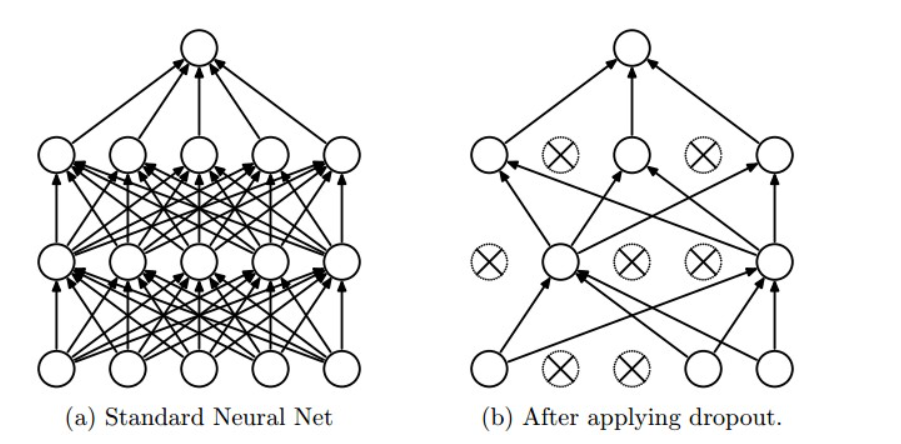
\includegraphics[width=0.7\textwidth]{dropout}
	\caption{dropout层}
\end{figure}

\subsubsection{前向传播}
根据上述定义便可以Dropout的前向传播代码进行编写,关键代码如下:
\begin{lstlisting}[language=python]
	if mode == "train":
		mask = (np.random.rand(*x.shape) >= p) / (1-p)
		out = x * mask
	elif mode == "test":
		out = x
	cache = (dropout_param, mask)
	out = out.astype(x.dtype, copy=False)
\end{lstlisting}



\subsubsection{反向传播}
后向传播时,训练阶段仅需要传播未mask的部分,关键代码如下:
\begin{lstlisting}[language=python]
	if mode == "train":
		dx = dout * mask
	elif mode == "test":
		dx = dout
\end{lstlisting}


\section{结果分析-BP神经网络}
	采用三层神经网络,结构为28 * 28 - 100 - 10进行下述实验探究。
\subsection{优化器的探究}
	采用早停法,设置在MNIST数据集迭代3次还没有验证集准确率的增加则停止,经过调试,对于SGD优化器,采用学习率0.02进行训练的效果较优;对于Adam优化器,采用学习率0.001训练效果较优,实验结果表格如下:
	\begin{table}[H]
	\centering
	\caption{实验结果表格}
	\begin{tabular}{|c|c|c|}
	\hline
	\textbf{Optimizer} & \textbf{SGD} & \textbf{Adam}  \\ \hline
	\textbf{val acc}   & 97.12        & \textbf{97.57} \\ \hline
	\textbf{Epoch}     & 36           & \textbf{14}    \\ \hline
	\end{tabular}
	\end{table}
	采用SGD优化器的训练损失下降图、验证准确率及训练准确率图如下:
	\begin{figure}[H]
		\centering
		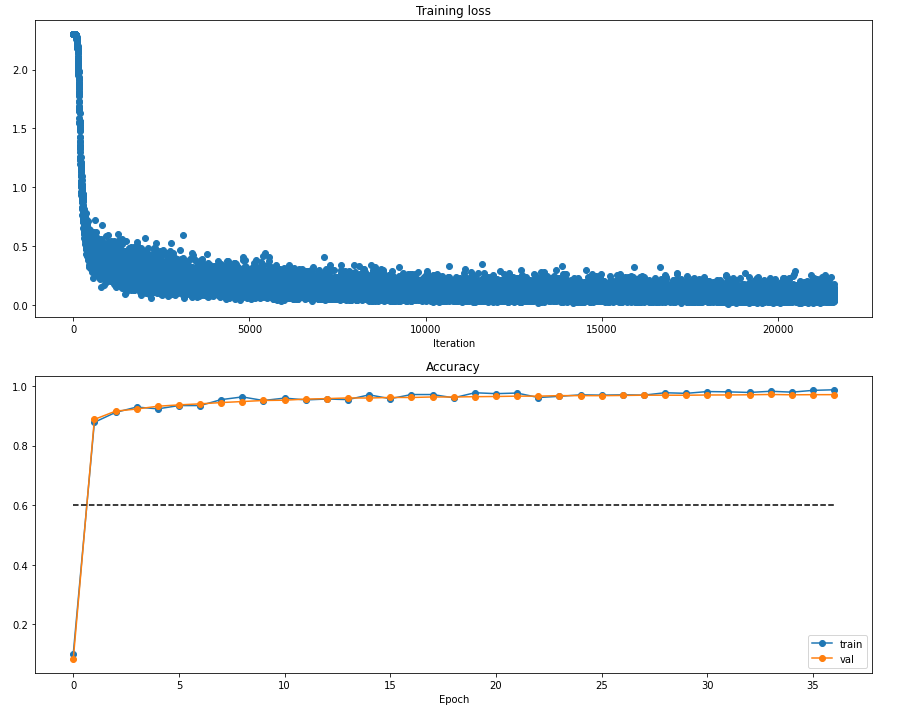
\includegraphics[width=0.5\textwidth]{sgd}
		\caption{实验结果}
	\end{figure}
采用Adam优化器的训练损失下降图、验证准确率及训练准确率图如下:
	\begin{figure}[H]
		\centering
		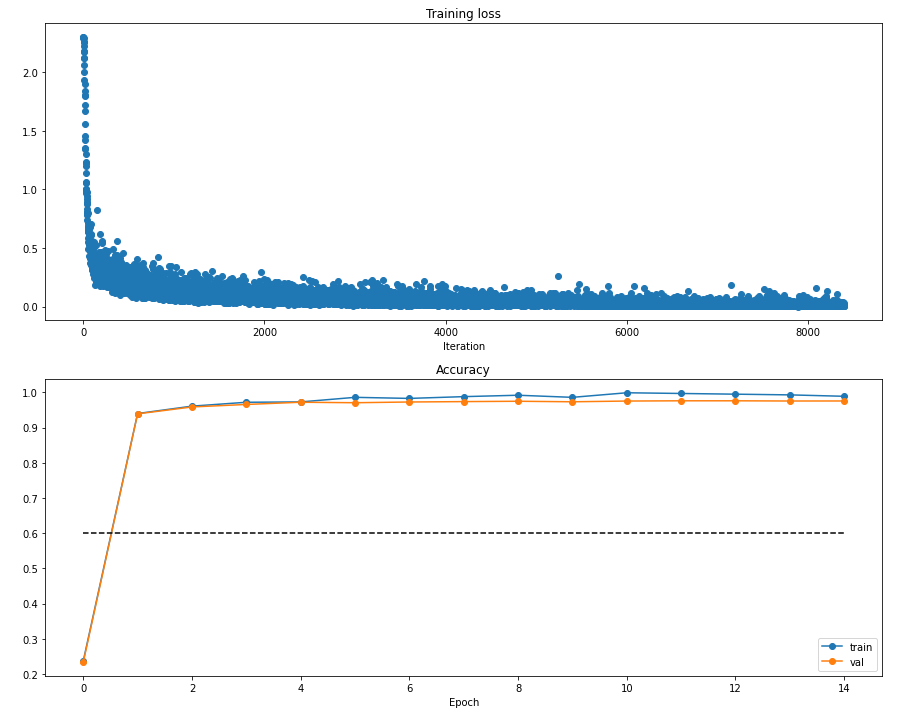
\includegraphics[width=0.5\textwidth]{adam}
		\caption{实验结果}
	\end{figure}

   从实验结果可得,使用Adam优化器相比SGD优化器对于BP网络的收敛速度和性能都有了很大的提升。


\subsection{对比批量归一化和丢弃法}

向BP网络中加入批量归一化和丢弃法,观察二者对于神经网络的影响,丢弃的概率选择0.5,结果如下:
\begin{table}[H]
\centering
\caption{实验结果}
\begin{tabular}{|c|c|c|c|c|}
\hline
\textbf{Model}   & \textbf{BPNN} & \textbf{BPNN+BN} & \textbf{BPNN+DP}     & \textbf{BPNN+BN+DP} \\ \hline
\textbf{val acc} & 97.62         & \textbf{97.91}   & 97.65       & 97.52      \\ \hline
\textbf{Epoch}   & 14            & 14               & \textbf{12} & 23         \\ \hline
\end{tabular}
\end{table}
结果显示,批量归一化和丢弃法单独使用时,都能够在准确率、迭代次数等方面使性能有所提升。然而,当二者同时使用时,BP网络的性能在准确率、迭代次数等方面都有所下降。
   
   
   
\section{结论-BP神经网络}
	在本次实验中,我们小组完成了三层BP网络的错误反传算法,实现了百分之70以上的准确率。同时,我们就优化器、批量归一化、丢弃法等BP神经网络常见优化方法进行了探究,发现如下结论:
	\begin{itemize}
	\item    从实验结果可得,使用Adam优化器相比SGD优化器对于BP网络的收敛速度和性能都有了很大的提升;
	\item 批量归一化和丢弃法单独使用时,都能够在准确率、迭代次数等方面使性能有所提升;
	\item 当批量归一化和丢弃法同时使用时,BP网络的性能在准确率、迭代次数等方面都有所下降。
	\end{itemize}
	其中第三点出现的原因我们推测为批量归一化在某种程度上防止过拟合的功能\cite{3}和丢弃法有所冲突,从而导致了BP网络的性能在准确率、迭代次数等方面性能的下降。
	

%hc 卷积神经网络的1.实验过程、2.结果分析和3.结论、


%\section{错误检测与恢复实验结果截图}
%\begin{figure}[H]
%	\centering
%	\includegraphics[width=1\linewidth]{errinput}
%	\caption{错误样例输入}
%\end{figure}
%\subsection{实验结果}
%\begin{figure}[H]
%	\centering
%	\includegraphics[width=1\linewidth]{cuowu}
%	\caption{错误检测与恢复实验结果}
%\end{figure}
%\begin{appendices}
%\end{appendices}
%
\begin{thebibliography}{99}
	\bibitem{1} Kingma D, Ba J. Adam: A method for stochastic optimization[C]//Proceedings of International
	Conference on Learning Representations. 2015.
%	
	\bibitem{2} Tieleman T, Hinton G. Lecture 6.5-rmsprop: Divide the gradient by a running average of its recent magnitude[Z]. 2012.
%	
	\bibitem{3} Ioffe S, Szegedy C. Batch normalization: Accelerating deep network training by reducing internal covariate shift[C]//Proceedings of the 32nd International Conference on Machine Learning. 2015:
	448-456.
	
	\bibitem{4} Srivastava N, Hinton G, Krizhevsky A, et al. Dropout: A simple way to prevent neural networks
	from overfitting[J]. The Journal of Machine Learning Research, 2014, 15(1):1929-1958.
\end{thebibliography}

\end{document}